\documentclass{article}
\usepackage[a4paper,total={7in,10in}]{geometry}
\usepackage[utf8]{inputenc}
\usepackage[colorlinks=true,citecolor=red]{hyperref}
\usepackage{graphicx}
\usepackage{amsmath,amssymb}
\usepackage{tikz}
\usetikzlibrary{backgrounds,fit}

\usepackage{longtable}
\LTcapwidth=180mm

\usepackage[tableposition=below]{caption}
\captionsetup[longtable]{skip=1em}

\begin{document}
\title{Documentation for FPGA-based digital PID controller}
\author{Ryan Thomas}

\maketitle

\section{Introduction}
This document is intended to describe how to use the FPGA-based digital PID controller included in this directory.  It will begin with an overview of the devices and their connections, then a description of the programmable logic, and finally a description of the two MATLAB classes used to control the device and some examples of their use.

Two different ISE project directories are included: ``Digital Servo Controller Single'' and ``Digital Servo Controller Quad''.  The ``single'' version is an FPGA architecture with a \emph{single} digital controller which uses the entire RAM for itself.  This means that it can record up to $4\times 10^6$ measurements from the ADC.  The ``quad'' version has \emph{four} independent controllers implemented within the FPGA logic, and each one gets one-fourth of the memory; therefore, each can store up to $10^6$ measurements from the ADC.  Due to time delays on SPI signals, you will need to use slower SPI clock frequencies with the quad controller compared to the single controller; for instance, use a 5 MHz SPI clock (200 ns period) with the quad control servos.  

\section{Devices}
\label{sec:Devices}
This section provides an overview of the different devices used with the controller as well as their configuration.

\subsection{FPGA}
\label{ssec:FPGA}
The controller uses a \href{https://numato.com/product/saturn-spartan-6-fpga-development-board-with-ddr-sdram}{Numato Labs Saturn Spartan 6 module} as the FPGA core of the device.  The Saturn module consists of a Xilinx Spartan 6 FPGA (part number XC6SLX45 CSG324-3) with 512 Mb of LPDDR RAM.  Interfacing with a computer is done through FTDI’s FT2232H dual-channel USB device.  An on-board 100 MHz oscillator provides the clock signal for the FPGA.  On-board SPI flash memory allows the FPGA bitstream to be downloaded directly using a USB cable and software provided by Numato Labs.

\subsubsection{Jumper configuration}
The Saturn module should be correctly configured out of the box.  Check on header P11 that jumpers are set between positions 1-2 and 5-6, and that on header P10 that jumpers are set on positions 1-2 and 5-6.  On header K1 (near the power plug), a jumper should connect the middle position and the position closest to the edge of the board.

\subsubsection{Driver installation}
Drivers for the FTDI chip can be found on \href{https://www.ftdichip.com/Drivers/D2XX.htm}{FTDI's website}.  Install the drivers, then plug in the FPGA.  You will also need to configure the USB chip so that channel B uses a serial connection.  Instructions for how to do this with a Windows computer can be found on Numato Lab's \href{https://numato.com/kb/configuring-ft2232h-usb-serial-converter-saturn-spartan-6-module/}{website}.

\subsubsection{Xilinx software}
While most of the code used in this project is VHDL, the project as a whole was created using Xilinx's ISE Design Suite 13.1.  The largest issue when moving to a different version of Xilinx's software is that some of the IP Cores, such as the multipliers, the digital clock management (DCM) blocks, and the memory interface generator, may need to be updated.  Additionally, ISE 13.1 does not function on Windows 10, and may not function at all on the latest macOS, so you may need to download virtual machine software and install a version of Linux on it to ensure compatibility.

\subsubsection{Uploading FPGA architecture}
Numato labs provides a utility for uploading FPGA architectures to the on-board SPI flash memory on the Saturn module, so you do not need any fancy cables.  This utility can be found on the downloads tab on the \href{https://numato.com/product/saturn-spartan-6-fpga-development-board-with-ddr-sdram}{Saturn webpage}.  A different version is included with the project called \verb|saturnflashconfig.exe|.  Once downloaded and with the Saturn module connected, open the program and click on the ``Load Binary File'' button.  Find the ``topmod.bin'' file in the appropriate project, and then click ``Program Flash''.  Occasionally the dialog will say that ``Programming failed...'', but if you click ``Program Flash'' again it will almost certainly program the device successfully on the second try.

\subsection{AD5791 evaluation board}
The actuator signal is the voltage created by an Analog Devices AD5791 20-bit digital-to-analog convertor (DAC).  To improve ease-of-use and performance, we use the EVAL-AD5791 evaluation board from Analog Devices.  It allows for communication via a serial-peripheral interface (SPI) compatible scheme and there is a header on the board that provides a breakout (header J6) for the necessary signals.  The board is powered from both $\pm15$ V (for the output analog circuitry) and $+5$ V for digital circuitry -- these are connected to the board using the two screw terminals.  The digital input/output voltage levels can be set with the voltage supplied to the IOVcc pin on the breakout header.

The evaluation board does not come with its own voltage reference, so you will need to either supply a $+5$ V reference or a $+10$ V and/or a $-10$ V reference.  The simplest solution is to provide a $+5$ V reference.  Depending on your application, you will want to have either a unipolar $0-10$ V output or a bipolar $-10$ to $10$ V output.  You should set the jumpers on the board as in Table~\ref{tb:DACJumper}.
\begin{table}[htbp]
	\centering
	\begin{tabular}{|l|p{10cm}|}
		\hline
		LK1 & Set to position B to source digital power supply from connector J2\\\hline
		LK3 & Set to position B to source digital voltage levels from pin 5 of J6\\\hline
		LK4, LK5, LK6 & Uninstall to pull up the $\overline{\text{LDAC}}$, $\overline{\text{CLR}}$, and $\overline{\text{RESET}}$ pins\\\hline
		LK8 & Set to position A to get $+5$ V voltage reference from connector VREF.\\\hline
		LK9 & Set to position B to get unipolar operation, or set to position C to get bipolar operation from $-10$ V to $10$ V.\\\hline
	\end{tabular}
	\caption{Header connections for the AD5791 evaluation board.}
	\label{tb:DACJumper}
\end{table}

While noise present in the DAC output is suppressed when used as part of a feedback loop, you will get better performance if you use a low-noise source.  However, for testing purposes the $+5$ V output from a normal power supply will suffice.

\subsection{ADS127L01 evaluation board}
Measurements are made using a Texas Instruments ADS127L01 24-bit analog-to-digital convertor (ADC) mounted on the manufacturer supplied evaluation board (ADS127L01EVM Rev. B).  The ADC can also be programmed using SPI once the Tiva microcontroller on the evaluation board has been disabled.  To power the device once without using USB, connect jumpers between JP1 and JP2 and disconnect the jumper on JP3.  You will then need to attach $+5$ V to pin 2 of JP3 and attach a ground to one of the GND test points.  Connect the rest of the headers as in Table~\ref{tb:ADCJumper}
\begin{table}[htbp]
	\centering
	\begin{tabular}{|l|p{10cm}|}
		\hline
		JP10, JP7, and JP5 & Disconnect these jumpers to enable the ADC, the initial differential amplifier, and the clock\\\hline
		JP8 & Connect a jumper between pin 2 and the pin labelled ``HR/LP''.\\\hline
		JP9 & Connect a jumper to enable the internal LDO for the LVDD supply\\\hline
		JP11 & Connect a jumper between the middle position (labelled DVDD) and the position labelled 3.3 V to set the logic level to 3.3 V.\\\hline
		JP6 & Connect a jumper across the pins labelled HR for high-resolution mode.\\\hline
	\end{tabular}
	\caption{Header connections for the ADC127L01 evaluation board (revision B).}
	\label{tb:ADCJumper}
\end{table}

In addition to the headers, the ADC has a number of settings that can be changed using the DIP switch S3.  Set these as in Table~\ref{tb:ADCsettings}.
\begin{table}[htbp]
	\centering
	\begin{tabular}{|l|l|}
		\hline
		$\overline{\text{HWEN}}$ & Set to 0 to use switch S3 to change ADC settings\\\hline
		HR & Set to 1 to use high-resolution mode\\\hline
		FORMAT & Set to 0 to use SPI for communication\\\hline
		FSMODE & Set to 0, although disabled when using SPI\\\hline
	\end{tabular}
	\caption{ADC settings using switch S3.}
	\label{tb:ADCsettings}
\end{table}
The filter settings are also changed using switch S3.  For a full description of the filter options, you should refer to the ADC data sheet.  Changing the filters will change the rate at which data is converted in the ADC and also the signal-to-noise ratio of that data.  Note that due to the overhead in the PID loop that the fastest data rate of 512 kSPS is not useable with the PID controller.  Our work has used the low-latency filter, which is accessed using $\text{FILTER[1:0]} = \text{0b10}$, with a 512x oversampling using $\text{OSR[1:0]} = \text{0b10}$.  With the on-board 16 MHz clock, this gives a sample rate of 31.25 kSPS.  


\section{Overview}
\label{sec:Overview}
The FPGA programmable logic is defined in behavioural terms using the VHDL language.  A schematic of the main components is shown in Fig.~\ref{fg:Components}.
\begin{figure}[htbp]
	\centering
	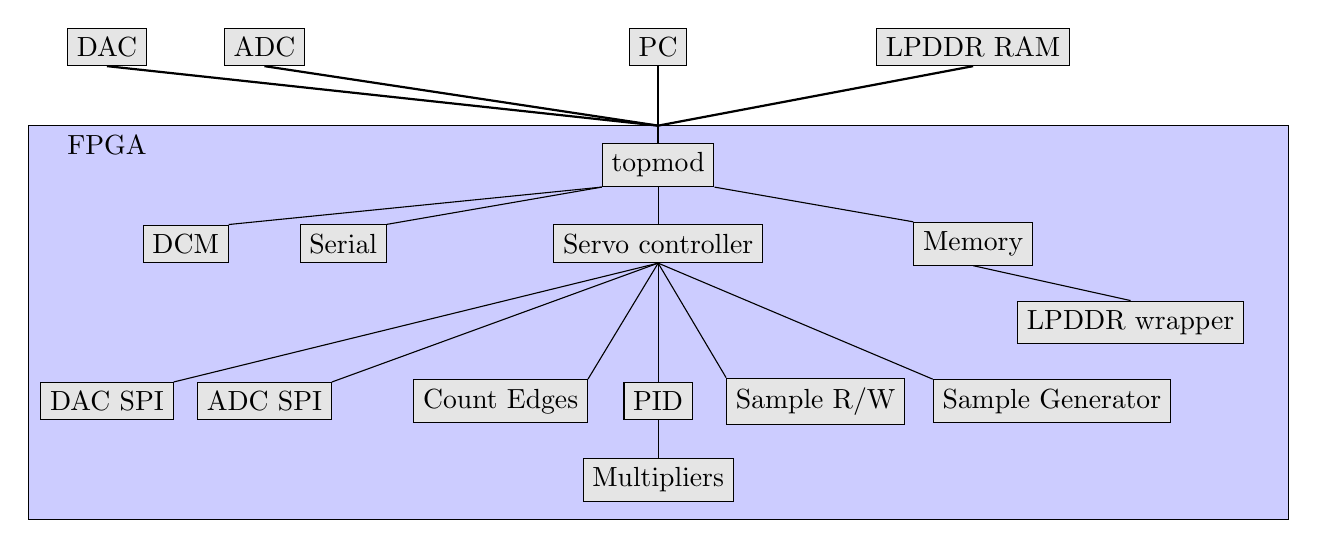
\begin{tikzpicture}[
		block/.style={draw,fill=gray!20!white}
		]
		%Draw FPGA
		\draw[fill=blue!20!white] (0,-0.5) rectangle (16,4.5);
		\path (8,4.5) coordinate (fpga);
		\path (1,4.5) node[below] {FPGA};
		\path (8,4) node[block] (topmod) {topmod}
		+(-6,-1) node[block] (dcm) {DCM}
		+(-4,-1) node[block] (serial) {Serial}
		+(4,-1) node[block] (memory) {Memory}
		+(0,-1) node[block] (control) {Servo controller}
		+(6,-2) node[block] (lpddr) {LPDDR wrapper}
		+(-7,-3) node[block] (dac) {DAC SPI}
		+(-5,-3) node[block] (adc) {ADC SPI}
		+(-2,-3) node[block] (count) {Count Edges}
		+(0,-3) node[block] (pid) {PID}
		+(2,-3) node[block] (memrw) {Sample R/W}
		+(5,-3) node[block] (sample) {Sample Generator}
		+(0,-4) node[block] (mult) {Multipliers};
		
		
		\draw (topmod.south west) -- (dcm.north east);
		\draw (topmod.south west) -- (serial.north east);
		\draw (topmod.south) -- (control.north);
		\draw (topmod.south east) -- (memory.north west);
		\draw (memory.south) -- (lpddr.north);
		\draw (control.south) -- (dac.north east);
		\draw (control.south) -- (adc.north east);
		\draw (control.south) -- (count.north east);
		\draw (control.south) -- (memrw.north west);
		\draw (control.south) -- (sample.north west);
		\draw (control.south) -- (pid.north);
		\draw (pid.south) -- (mult.north);
		%Draw external components
		\path (1,5.5) node[block] (DAC) {DAC}
		+(2,0) node[block] (ADC) {ADC}
		+(7,0) node[block] (pc) {PC}
		(12,5.5) node[block] (ram) {LPDDR RAM};
		\draw[thick] (topmod.north) -- (fpga.south);
		\draw[thick] (fpga.north) -- (DAC.south);
		\draw[thick] (fpga.north) -- (ADC.south);
		\draw[thick] (fpga.north) -- (pc.south);
		\draw[thick] (fpga.north) -- (ram.south);
	\end{tikzpicture}
	\caption{Diagram of the different components comprising the FPGA programmable logic and outside connections.}
	\label{fg:Components}
\end{figure}
The module ``topmod'' is the top-most level and it is what connects to the physical world through its input and output pins.  Within topmod there are four different components: the digital clock management (DCM), the serial interface, the memory controller, and the actual servo controller.

\subsection{Top level components}
\label{ssec:topLevelComponents}
The DCM takes the 100 MHz on-board clock and generates a phase-locked internal 100 MHz clock used for clocking the LPDDR RAM and a 50 MHz clock for clocking everything else.  

\begin{figure}[htbp]
	\centering
	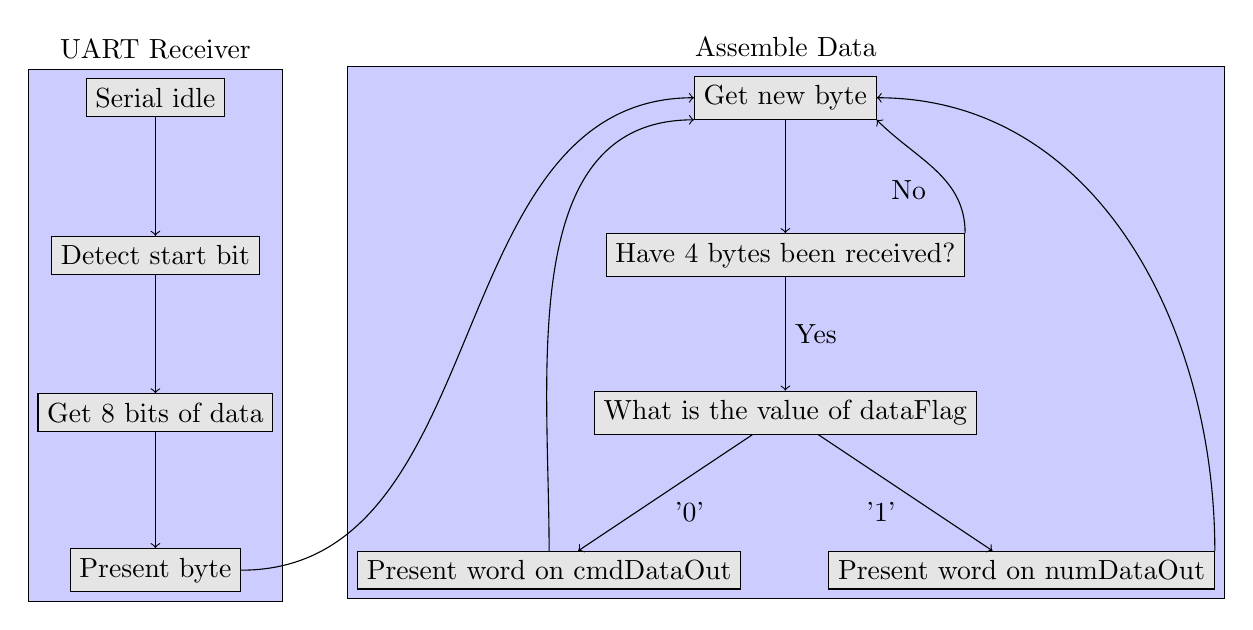
\begin{tikzpicture}[
		block/.style={draw,fill=gray!20!white},
		auto
		]
		\path (0,0) node[block] (idle) {Serial idle}
		 ++(0,-2) node[block] (start bit) {Detect start bit}
		 ++(0,-2) node[block] (get bits) {Get 8 bits of data}
		 ++(0,-2) node[block] (receive done) {Present byte};
		\draw[->] (idle) -- (start bit);
		\draw[->] (start bit) -- (get bits);
		\draw[->] (get bits) -- (receive done);
		
		\path (8,0) node[block] (get byte) {Get new byte}
		++(0,-2) node[block] (is done) {Have 4 bytes been received?}
		++(0,-2) node[block] (dataFlag) {What is the value of dataFlag}
		++(-3,-2) node[block] (cmd out) {Present word on cmdDataOut}
		++(6,0) node[block] (num out) {Present word on numDataOut};
		
		\draw[->] (receive done.east) to[out=0,in=180] (get byte.west);
		\draw[->] (get byte) -- (is done);
		\draw[->] (is done) to node {Yes} (dataFlag);
		\draw[->] (is done.north east) to[out=90,in=-45] node {No} (get byte.south east);
		\draw[->] (dataFlag) to node {'0'} (cmd out);
		\draw[->] (dataFlag) to node[swap] {'1'} (num out);
%		\draw[->] (cmd out) -- (reset);
%		\draw[->] (num out) -- (reset);
%		\draw[->] (reset) to[out=0,in=0] (get byte);
		\draw[->] (cmd out) to[out=90,in=180] (get byte.south west);
		\draw[->] (num out.north east) to[out=90,in=0] (get byte.east);
		
		\begin{scope}[on background layer]
			\node[draw,fill=blue!20!white,fit=(idle) (start bit) (get bits) (receive done),label=UART Receiver] (fillReceive) {};
			\node[draw,fill=blue!20!white,fit=(get byte) (is done) (dataFlag) (cmd out) (num out),label=Assemble Data] {};
%			\node[above] (fillReceive.north) {UART Receiver};
		\end{scope}

	\end{tikzpicture}
	\caption{Flow chart of serial interface.}
	\label{fg:SerialFlowChart}
\end{figure}
The serial interface handles communication with the PC using the universal asynchronous receiver/transmitter protocol with a baud rate of 1 MHz.  While the FTDI chip can handle baud rates of up to 12 MHz, a rate of 1 MHz was chosen as being the fastest rate with the minimum of lost bytes during transmission.  Higher baud rates do not seem to work well, and if faster transmission is required a different protocol should be used.  The serial interface assumes that data will be sent in one byte at a time with 1 start bit, 1 stop bit, and no parity bits.  Each complete transmission should be four bytes starting with the least-significant byte, and within each byte the data should be sent least-significant bit first.  When four bytes have been received, the complete 32-bit word is presented on one of two output signals and a data ready flag is raised for one clock cycle.  The assumption behind the serial interface in the FPGA is that most data will be sent first as a 32-bit address and then (possibly) a 32-bit data word.  For some commands, such as a software start trigger, it is necessary to send only the address.  A flow chart of incoming serial data is processed is shown in Fig.~\ref{fg:SerialFlowChart}.  In case a data byte has been lost, the serial interface resets itself after $10^5$ baud periods, or 100 ms, if it has not received four bytes in that time.

The memory controller module acts as a simple interface for the LPDDR interface created by Xilinx's Memory Interface Generator.  It is suitable for low rates of reading and writing.  It is essentially just two state machines that handle read and write requests.  A write request is initiated by presenting a 28-bit address, a 32-bit data word to be written, and a write trigger signal that should be high for one 50 MHz clock cycle.  The state machine takes care of writing data to the memory.  For simplicity, no writes can take place while read operations are occurring -- they will simply be paused until the read operation is complete.  A read operation is started by presenting a 28-bit address and a read trigger to the controller.  Once the data has been retrieved, it is presented on the output of the memory controller along with a data valid signal that is high for one clock cycle.

\subsection{Servo controller components}
\label{ssec:servoControllerComponents}
The servo controller consists of a number of different components and processes along with combinatorial logic.  Most of these components are interdependent on each other.  A normal sequence for running the servo controller might be as follows.  First, a start signal is received either from the serial interface as a specific command or as the rising edge of an external pin.  This start signal starts the reading of ADC data using the ADC SPI component.  Depending on various settings, this data may be written to memory using the Sample R/W component.  At the same time, the sample generator starts.  Depending on the sample source, new samples are either created on-the-fly using piece-wise linear ramps or they are read from RAM.  Each sample value is associated with an 8-bit sample code; currently only the least-significant bit is used.  When this LSB is 0, the corresponding sample is interpreted as a control signal and both this and the measurement signal from the ADC are passed to the PID component which calculates the next value for the DAC.  If the sample code's LSB is 1, then the sample is interpreted as a value to be written \emph{directly} to the DAC.  This means that the PID process is disabled for this sample.  The process continues until the sample generator determines that it has produced as many samples as requested, and data is collected and sent to memory for this period.

A separate process in the servo controller module keeps track of the total time since the start signal.  When this value reaches a so-called ``off time'' then the DAC values from either the PID component or directly from the sample generator are overridden and an ``off value'' is written to the DAC.  This is useful because it may be that one wants to switch off the DAC output with a time resolution better than that achieved using the sample generator.  The ``off value'' is programmable to account for systems that may require a voltage different than 0 V to switch off.  After a hold off period a reset command is sent to the sample generator which stops it and resets its state.

Data that was saved to the RAM during this sequence can be retrieved using the serial interface.  Data from the RAM is read out as one block -- a command is sent to read data and it is streamed as fast as possible to the host computer.  As significant amounts of data can be stored, and the serial interface has a limited speed, a starting and ending sample can be specified as well as a sample step size.  This allows the user to retrieve only the data range of interest.

The servo controller component defines four constants related to locations in memory.  These are listed in Table~\ref{tb:memoryLocations}.  All memory locations accessed in the servo controller are 28 bits long and the four most-significant bits are always 0b0000.  The next two most-significant bits define what is stored in memory, and the rest of the bits define which sample is being accessed.
\begin{table}[htbp]
	\centering
	\begin{tabular}{|l|l|l|}
		\hline
		\verb+SAMPLE_LOCATION+ & 0b00 & Location of sample values\\\hline
		\verb+LOOP1_LOCATION+ & 0b01 & Location of the first loop register comprised of $(K_i,K_p)$.\\\hline
		\verb+LOOP2_LOCATION+ & 0b10 & Location of the second loop register comprised of $(N,K_d)$.\\\hline
		\verb+DATA_LOCATION+ & 0b11 & Location of saved measurement data.\\\hline
	\end{tabular}
	\caption{Table of memory locations.  See Eq.~\eqref{eq:controlLaw} for descriptions of the loop registers.}
	\label{tb:memoryLocations}
\end{table}

\subsubsection{SPI drivers}
\label{sssec:SPI}
The FPGA communicates with both the DAC and the ADC using SPI, and the functionality is encapsulated in the \verb+SPI_DRIVER+ component.  Although the driver can read and write data at the same time, the DAC driver operates only in write mode and the ADC driver operates only in read mode.  SPI has four different modes of operation which relate to the polarity of the clock signal and the edge of the clock signal on which data is written/read from the slave device.  In the driver module, the CPOL generic sets the idle polarity of the SCLK (serial clock) signal: if CPOL is 0, then the idle polarity of SCLK is 0, and if CPOL is 1 then the idle polarity is 1.  The CPHA generic controls the edge on which data is clocked into or out of the device.  If CPHA is 0, the data is valid on the $\text{CPOL}\rightarrow\overline{\text{CPOL}}$ transition, and if CPHA is 1 data is valid on the opposite transition.

The driver only operates when the enable signal is high.  A write cycle proceeds when the driver is idle (output port \verb+busy+ is low), data is present on the \verb+dataToSend+ input port, and a the driver receives a trigger.  If the trigger is an external signal that is not necessarily synchronized with the FPGA clock, then there is a generic option to create a synchronized signal on either the rising or falling edge of the input trigger.  When the trigger is received, the SYNC signal is pulled to its active level (low for both the DAC and the ADC), the serial clock is started at the given \verb+spiPeriod+, and data is sent to the device in accordance with the CPOL and CPHA parameters.  After the final bit of data has been transmitted, the SYNC signal is pulled to its non-active level (high for the DAC and the ADC).  An input signal, \verb+syncDelay+, can be used to delay this final transition of the SYNC signal.  While not needed for the AD5791, if a different DAC is used -- such as the MAX5719 -- a delay between the final bit and the SYNC edge may be needed.  In the servo controller, triggers for the DAC process are all internal triggers.

The read process occurs in much the same way as the write process.  For the servo controller, the start trigger for the SPI process is the falling edge of the $\overline{\text{DRDY}}$ signal from the ADC.  Once this edge is registered, the serial clock starts and data from the ADC is clocked in on the appropriate edge.  Once all data has been received, the assembled data word is presented on the output of the driver and a data ready signal is raised high for one FPGA clock cycle.

\subsubsection{Count edges}
\label{sssec:countEdges}
The Count Edges component is quite simple: it counts the number of clock cycles between either rising or falling edges of its \verb|edgeIn| signal.  This component is used to determine the ADC sample rate using the \verb|ADC_DRDY| signal and report it back to the PC.  It can be a useful diagnoses for issues with the ADC clock.

\subsubsection{Sample Generator}
\label{sssec:SampleGenerator}
The sample generator component either calculates new samples as piecewise linear ramps or retrieves these values from memory.  The component consists of three processes: Update, LinearRamp, and MemoryRamp.  The Update process increments the sample counter and delays new samples by the input signal \verb+updateTime+.  On the receipt of a trigger, the generator's enable signal is set to high which is used by other components in the servo controller.  The process then loads the appropriate sample data into its active registers depending on the input signal \verb+sampleSource+: if `0', then new samples come from LinearRamp, and if `1' then new samples come from MemoryRamp.  An update trigger is then raised high for one clock cycle which indicates to other components that a new sample is valid.  The Update process then waits for the time \verb+updateTime+ before retrieving the next sample.  This process continues until the sample count exceeds the user-specified input signal \verb+numSamples+.

The LinearRamp process calculates new output samples using three arrays of integers: \verb+rampValues+, \verb+rampBndyTimes+, and \verb+rampRates+.  At the start of a sequence, the first sample value is \verb+rampValues(0)+ and the ramp index \verb+rampIdx+ is set to 0.  On each update trigger, the sample count is checked against the values of the array of \verb+rampBndyTimes+ which define the \emph{boundary times} of the linear ramps.  If the sample count is equal to the boundary time corresponding to the current ramp index, then the output sample is set to \verb+rampValue(rampIdx)+.  When the sample count is less than the boundary time corresponding to the \emph{next} ramp, then the corresponding \verb+rampRate+ is added to the current value of the output sample.  The ramp index is incremented when the sample count is equal to the next boundary time \emph{minus 1}.

The MemoryRamp process retrieves new samples from memory as well as new loop parameters.  When the process receives an update trigger, it calculates the appropriate memory address from the sample count to retrieve the new sample.  The process then waits for the memory controller to indicate that new data is ready before reading that data in.  Sample values are interpreted as the least significant 24 bits of the 32-bit data word, and sample codes are the 8 most-significant bits.  The controller then reads the updated values for the PID controller into the \verb+loopReg1+ and \verb+loopReg2+ signals, both of which are 32-bits wide.  The MemoryRamp process knows where to retrieve the sample and loop data due to generics in its instantiation.   Additionally, this process reads the first sample on the receipt of a reset signal which means that the first sample is always immediately available to the Update process when a sequence is first started.

In addition to sample values, the user provides \emph{sample codes} to either the linear ramp or arbitrary ramp generators.  The sample code is an 8-bit word that can control the sample process.  Currently only two bits are used.  The least-significant bit (LSB) controls whether or not the servo controller should consider the new sample value to be an ADC value to stabilise to ($\mathrm{LSB}=0$) or a DAC value that should be directly written to the DAC ($\mathrm{LSB}=1$). 

 When using arbitrary ramps retrieved from memory, there is also the possibility of \emph{compressing} the sample values in the situation when the sample is held at a particular value for a long period of time.  For instance, if one is using the servo to control the current in a magnetic trap that will be held at a particular current for 10 s, then rather than writing 312500 samples to the memory one can write just \emph{two} values: the value itself and how many samples to hold for.  This hold phase is enabled by writing a sample where the sample code's most-significant bit is `1' and the sample value is the number of update cycles to delay for.

\subsubsection{Sample R/W}
\label{sssec:sampleRW}
This module has two purposes: it records sample data on each edge and keeps track of how many samples have been recorded, and it streams data back to the PC when requested.  When the module gets a \verb|dataReady| signal, it issues a write request to the memory controller with the new data and an address composed of the current sample count and the appropriate memory location, in this case \verb|DATA_LCOATION|.  At the same time, it updates a counter called \verb|sampleCountMax| that keeps track of how many samples have been recorded so that when reading samples back the entire memory is not read.

When reading data, the controller has four different read modes: data, sample, loop 1, or loop 2, each corresponding to a different memory location as specified in Table~\ref{tb:memoryLocations}.  Data is streamed directly to the host computer.  To limit the amount of data, the user can enable the \verb|useSampleLimits| signal and set the minimum and maximum sample counts to retrieve (inclusive) and the step size to take.  To check for errors, the controller will also calculate the signal \verb|numRequestedSamples| which can be read using the serial interface and is useful for checking for missing samples that may have been lost during transmission using the serial interface.

\subsubsection{PID}
The PID module is what actually implements the proportional-integral-derivative control law.  The module calculates a new actuator value $u_n$ at time step $n$ according to
\begin{equation}
u_n = u_{n-1}+2^{-N}\left[K_p\underset{\text{propTerm}}{\underbrace{(e_n-e_{n-1})}}+\frac{K_i}{2}\underset{\text{integralTerm}}{\underbrace{(e_{n}+e_{n-1})}}+K_d\underset{\text{derivativeTerm}}{\underbrace{(e_n-2e_{n-1}+e_{n-2})}}\right]
\label{eq:controlLaw}
\end{equation}
where $e_n = r_n - y_n$ is the error signal, $K_p$, $K_i$, $K_d$ are the proportional, integral, and derivative gains, respectively, $N$ is an overall divisor used to rescale the gains to approximate arbitrary values, $r_n$ is the control signal, and $y_n$ is the measurement value.  The controller can use either fixed gain and divisor values, or it can use variable values obtained from the sample generator.  The fixed gains are input using the signal \verb|loopRegFixed|, and the variable gains are input using \verb|loopRegVary|.  Both registers are 64-bits wide, and each of the gains and the divisor are 16 bits wide.  The encoding in the registers is, from most-significant bit to least-significant, $(N,K_d,K_i,K_p)$.  For the servo controller, the actuator value is the voltage code for the DAC, the measurement is the voltage code from the ADC, and the control signal is a voltage code corresponding to the ADC encoding.

On the receipt of a \verb|measReady| signal, the PID module parses the appropriate loop register depending on the value of \verb|useFixed|, and it also calculates the values of $\text{propTerm}$, $\text{integralTerm}$, and $\text{derivativeTerm}$ and stores the last two values of the error signal.  The error signal itself is calculated using combinatorial logic as \emph{either} $e_n = r_n-y_n$ for the normal, negative polarity PID controller, or as $e_n = y_n - r_n$ for positive polarity.  Positive polarity control is needed in situations where a positive change in the actuator signal causes a negative change in the measurement.  The main process then waits for seven clock cycles to let the multipliers compute the new values and provide updated results.  Once multipliers have produced updated values, the sum $K_p(\text{propTerm})+K_i(\text{integralTerm})/2+K_d(\text{derivativeTerm})$ is used to increment the 56-bit wide signal \verb|pidDivide|.  \verb|pidDivide| is clipped at maximum and minimum values provided using the serial interface before being shifted right by $N$ bits to approximate division by $2^N$.  It is necessary that the division occurs after summation in order to eliminate round-off errors.  This shifted value is then converted from a signed integer into an unsigned integer appropriate for the DAC by adding it to a \verb|dacZero| signal and then converting it to the appropriate width.  At the end of the process, a \verb|trigOut| signal is raised high for one clock cycle to indicate that the output signal is now valid.

\section{Use}
\label{sec:Use}
This section describes how to use the controller, in terms of connections to the FPGA, how parameters are encoded, and how to use the MATLAB classes.  It concludes with examples of how to program the device.

\subsection{Connections}
\label{ssec:connections}
The physical pins that each internal signal of the FPGA is connected to can be found in the constraints file of the project.  Below is a summary of these connections.  For the ``single'' version of the FPGA architecture, connect signals as for ``Servo 2''.
%\begin{longtable}[c]{|l|p{8cm}|l|}
%		\hline
%		\textbf{Name} 			&\textbf{Description}										&\textbf{Pin on Saturn module}\\\hline
%		\verb|IOVcc|			&3.3 V power on FPGA, connect to IOVcc on DAC				&P2-3\\\hline
%		\verb|GND|				&Ground on FPGA, connect to GND on DAC						&P2-7\\\hline
%		\verb|DAC_SCLK|			&DAC serial clock, connect to SCLK on DAC					&P2-11\\\hline
%		\verb|DAC_SDOUT|		&DAC serial data out, connect to SDIN on DAC				&P2-15\\\hline
%		\verb|DAC_LDAC|			&DAC load DAC signal, connect to LDAC on DAC				&P2-19\\\hline
%		\verb|DAC_SYNC|			&DAC serial SYNC or CE signal, connect to SYNC on DAC		&P2-23\\\hline
%		\verb|DAC_SWITCH|		&Switch signal.  If you have an external switch for the DAC voltage, connect to this.		&P2-27\\\hline
%		\hline
%		\verb|GND|				&FPGA ground, connect to GND on ADC.						&P2-4\\\hline
%		\verb|ADC_SDOUT|		&ADC serial data out, connect to DIN on ADC					&P2-8\\\hline
%		\verb|ADC_SCLK|			&ADC serial clock, connect to SCLK on ADC					&P2-12\\\hline
%		\verb|ADC_SDIN|			&ADC serial data in, connect to DOUT on ADC					&P2-16\\\hline
%		\verb|ADC_DRDY|			&ADC data ready, connect to DRDY on ADC						&P2-20\\\hline
%		\verb|ADC_START|		&ADC start signal.  Leave unconnected						&P2-24\\\hline
%		\verb|ADC_SYNC|			&ADC serial SYNC signal, connect to SYNC on ADC				&P2-28\\\hline
%		\hline
%		\verb|extStartTrig|		&External start signal.  Connect to an external, 3.3 V logic start signal					&P3-85\\\hline
%		\verb|EXT_SWITCH|		&External switch input signal.  Use if you want to have an external signal control the DAC switch and have its falling edge switch off the controller					&P3-86\\\hline
%%		\caption{FPGA connections to the DAC and ADC.}
%%		\label{tb:connections}
%\end{longtable}
\begin{longtable}[c]{|l|p{7cm}|l|l|l|l|}
	\hline
	\textbf{Name} 			&\textbf{Description}										&\multicolumn{4}{c|}{\textbf{Pin on Saturn module}}\\\hline
							&															&\textbf{Servo 0}	&\textbf{Servo 1}	&\textbf{Servo 2}	&\textbf{Servo 3}\\\hline
	\verb|IOVcc|			&3.3 V power on FPGA, connect to IOVcc on DAC				&\multicolumn{4}{c|}{Connect to a Vcc pin, such as P2-3}\\\hline
	\verb|GND|				&Ground on FPGA, connect to GND on DAC						&\multicolumn{4}{c|}{Connect to a GND pin, such as P2-7}\\\hline
	\verb|DAC_SCLK|			&DAC serial clock, connect to SCLK on DAC					&P3-26				&P3-28				&P2-11				&P3-87\\\hline
	\verb|DAC_SDOUT|		&DAC serial data out, connect to SDIN on DAC				&P3-22				&P3-24				&P2-15				&P3-83\\\hline
	\verb|DAC_LDAC|			&DAC load DAC signal, connect to LDAC on DAC				&P3-14				&P3-16				&P2-19				&P3-79\\\hline
	\verb|DAC_SYNC|			&DAC serial SYNC or CE signal, connect to SYNC on DAC		&P3-18				&P3-20				&P2-23				&P3-75\\\hline
	\verb|DAC_SWITCH|		&Switch signal.  If you have an external switch for the DAC voltage, connect to this.				&P3-10				&P3-12				&P2-11				&P3-71\\\hline
	\hline
	\verb|GND|				&FPGA ground, connect to GND on ADC.						&\multicolumn{4}{c|}{Connect to a GND pin, such as P2-7}\\\hline
	\verb|ADC_SDOUT|		&ADC serial data out, connect to DIN on ADC					&P3-13				&P3-15				&P2-8				&P3-88\\\hline
	\verb|ADC_SCLK|			&ADC serial clock, connect to SCLK on ADC					&P3-17				&P3-19				&P2-12				&P3-84\\\hline
	\verb|ADC_SDIN|			&ADC serial data in, connect to DOUT on ADC					&P3-9				&P3-11				&P2-16				&P3-80\\\hline
	\verb|ADC_DRDY|			&ADC data ready, connect to DRDY on ADC						&P3-5				&P3-7				&P2-20				&P3-76\\\hline
	\verb|ADC_START|		&ADC start signal.  Leave unconnected						&P3-25				&P3-27				&P2-24				&P3-72\\\hline
	\verb|ADC_SYNC|			&ADC serial SYNC signal, connect to SYNC on ADC				&P3-21				&P3-23				&P2-28				&P3-64\\\hline
	\hline
	\verb|extStartTrig|		&External start signal.  Connect to an external, 3.3 V logic start signal					&P3-29		&P3-31		&P3-85		&P3-63\\\hline
	\verb|EXT_SWITCH|		&External switch input signal.  Use if you want to have an external signal control the DAC switch and have its falling edge switch off the controller		&P3-30	&P3-32	&P3-86	&P3-59\\\hline
	\caption{FPGA connections to the DAC and ADC.}
	\label{tb:connections}
\end{longtable}

\subsection{Parameter addresses and encoding}
\label{ssec:parameters}
The controller has a number of different parameters that need to be set appropriately for it to work as desired.  All of these parameters are accessed using the serial interface.  A table of parameters, including their address, data type, and use, is shown in Table~\ref{tb:Parameters}.  The two most-significant address bits are reserved for use as a controller ID, although this is not implemented in the single controller version and thus these bits can be anything.  The next two address bits are used to determine whether to read/write data to a parameter or to memory.  Their encoding is:
\begin{itemize}
	\item $00 \rightarrow \text{write parameter}$
	\item $01 \rightarrow \text{write to memory}$
	\item $10 \rightarrow \text{read parameter}$
	\item $11$ not used.
\end{itemize}
Most parameters are written to using a two step procedure.  First, an address is sent over serial to the FPGA.  Second, some kind of numerical data is sent over.  How the numerical data is parsed in the FPGA is indicated in the ``Numerical data type'' column of Table~\ref{tb:Parameters}.  Parameters where that column is ``null'' are those where numerical data does not need to be sent; typically, these are trigger signals for which numerical data is unnecessary.  Numerical data should be aligned with the least-significant bit, so a 16-bit parameter sent over serial as 32 bits should be 0bxxxx xxxx xxxx xxxx dddd dddd dddd dddd where x is ``don't care'' and d are data bits.

\begin{longtable}[c]{|l|l|l|p{6cm}|}
	\hline
	\textbf{Name} 			&\textbf{Address}			&\textbf{Numerical data type} 				&\textbf{Description}\\
	\hline
	
	\multicolumn{4}{|c|}{\textbf{Manual parameters}}\\
	\hline
	\verb|manDataDAC|		&0x00 00 00 xx				&24-bit \verb|std_logic_vector|	&24 bits to send directly to the DAC.  Used for setting up the DAC and setting the DAC voltage manually.\\\hline
	\verb|manTrigDAC|		&0x00 00 01 xx				&null							&Tells the controller to trigger the DAC SPI.\\\hline
	\verb|manSwitchDAC|		&0x00 00 02 (00,01)			&null							&Manually sets the switch signal (if used).  If the LSB of the address is 0 then the switch signal is low, if the LSB is 1 then the 																				switch signal is high.\\\hline
	\verb|manTrigADC|		&0x00 00 03 xx				&null							&Tells the controller to manually trigger the ADC to collect \verb|numSamples| samples of data.  Useful for debugging.\\\hline
	
	\multicolumn{4}{|c|}{\textbf{Software triggers}}\\
	\hline
	\verb|resetMan|			&0x01 00 00 xx				&null							&Issues a reset command to the sample generator.\\\hline
	\verb|manTrigRamp|		&0x01 00 01 xx				&null							&Issues a start trigger to the ramp generator.  A software trigger for the sequence.\\\hline
	\verb|startTransmit|	&0x01 00 02 (00,01,10,11)	&null							&Tells the sample R/W module to start reading back data from memory and sending to the host computer using serial.  The last two 	bits of the address indicate which data to access, and these correspond to the memory locations in Table~\ref{tb:memoryLocations}.\\\hline
	
	\multicolumn{4}{|c|}{\textbf{Global parameters}}\\
	\hline
	\verb|spiPeriod|		&0x02 00 00 xx				&unsigned 31-bit integer		&Number of clock cycles between rising edges of the SCLK for both the ADC and the DAC.\\\hline
	\verb|transmitType|		&0x02 00 01 xx				&unsigned integer [0,3]			&Type of data to save to memory and then transmit.  0: ADC data, 1: DAC output, 2: control signal, 3: error signal.\\\hline
	\verb|enableTrig|		&0x02 00 02 xx				&\verb|std_logic|				&Set to high to enable external trigger.  This signal is set to 0 on power up to prevent the controller from running without being programmed.\\\hline
	\verb|offTime|			&0x02 00 03 xx				&unsigned 32-bit integer		&Number of clock cycles before the switch is shut and the override DAC process starts.\\\hline
	\verb|ADC_START|		&0x02 00 04 (00,01)			&null							&Sets the value of the \verb|ADC_START| signal, which can be connected to the START pin on the ADC to synchronize the start of conversions if using more than one ADC.\\\hline
	\verb|samplePeriodADC|	&0x02 00 05 xx				&null							&Read-only parameter.  Tells the controller to send over serial the current ADC sample period as measured using the Count Edges module.\\\hline
	
	\multicolumn{4}{|c|}{\textbf{DAC settings}}\\
	\hline
	\verb|minValueDAC|		&0x03 00 00 xx				&unsigned 20-bit integer		&Minimum DAC code allowed.  DAC codes corresponding to smaller values will be clipped.\\\hline
	\verb|maxValueDAC|		&0x03 00 01 xx				&unsigned 20-bit integer		&Maximum DAC code allowed.  DAC codes corresponding to larger values will be clipped.\\\hline
	\verb|syncDelay|		&0x03 00 02 xx				&unsigned 8-bit integer			&Delay between last bit written to DAC and rising edge of SYNC, in clock cycles.\\\hline
	\verb|dacMode|			&0x03 00 03 xx				&\verb|std_logic|				&Polarity of DAC.  `0' corresponds to unipolar operation, and `1' to bipolar operation.\\\hline
	\verb|dacOffValue|		&0x03 00 04 xx				&20-bit \verb|std_logic_vector|	&DAC code corresponding to the code the DAC should have when the servo is ``off''. Written to DAC at \verb|offTime|\\\hline
	\verb|useExternalSwitch|&0x03 00 05 xx				&\verb|std_logic|				&Uses an external switch line to control both the switch output from the FPGA and the DAC override process.  If enabled, the \verb|DAC_SWITCH| signal will be high only when \verb|EXT_SWITCH| is also high, and the override process will start on the falling edge of the \verb|EXT_SWITCH| line.\\\hline
	
	\multicolumn{4}{|c|}{\textbf{Sample generator settings}}\\
	\hline
	\verb|sampleSource|		&0x04 00 00 xx				&\verb|std_logic|				&Selects the sample source.  `0' is for piece-wise linear ramps, and `1' draws samples from RAM.\\\hline
	\verb|updateTime|		&0x04 00 01 xx				&unsigned 31-bit integer		&Number of clock cycles between successive samples.\\\hline
	\verb|numSamples|		&0x04 00 02 xx				&unsigned 31-bit integer		&Number of samples to write in automatic mode, or number of ADC samples to collect when manually triggered using \verb|manTrigADC|.\\\hline
	
	\multicolumn{4}{|c|}{\textbf{Linear ramp settings}}\\
	\hline
	\verb|rampValues|		&0x05 00 00 $ii$				&32-bit signed integer		&Sets the starting value for each linear ramp.  $ii$ indicates the ramp index to write to.  $ii \in [0,7]$\\\hline
	\verb|rampBndyTimes|	&0x05 00 01 $ii$				&32-bit signed integer		&Sets the boundary time for each linear ramp.  $ii$ indicates the ramp index to write to.  $ii \in [0,7]$\\\hline
	\verb|rampRates|		&0x05 00 02 $ii$				&32-bit signed integer		&Sets increment to add at each update time to change the ramp value.  $ii$ indicates the ramp index to write to.  $ii \in [0,6]$\\\hline
	\verb|rampCodes|		&0x05 00 03 $ii$				&8-bit unsigned integer		&Sets the ramp code for each linear ramp.  $ii$ indicates the ramp index to write to.  $ii \in [0,7]$\\\hline
	
	\multicolumn{4}{|c|}{\textbf{PID settings}}\\
	\hline
	\verb|polarity|			&0x06 00 00 xx					&\verb|std_logic|			&PID polarity.  `0' is negative, `1' is positive.\\\hline
	\verb|Kp|				&0x06 00 01 xx					&16-bit unsigned integer	&Value of the proportional gain.\\\hline
	\verb|Ki|				&0x06 00 02 xx					&16-bit unsigned integer	&Value of the integral gain.\\\hline
	\verb|Kd|				&0x06 00 03 xx					&16-bit unsigned integer	&Value of the derivative gain.\\\hline
	\verb|divisorPID|		&0x06 00 04 xx					&16-bit unsigned integer	&Overall divisor for the PID process.  See Eq.~\eqref{eq:controlLaw}.\\\hline
	\verb|useFixed|			&0x06 00 05 xx					&\verb|std_logic|			&Set to `0' to use variable loops, and set to `1' to use fixed gain loops.\\\hline
	
	\multicolumn{4}{|c|}{\textbf{Memory settings}}\\
	\hline
	\verb|numMemSamples|	&0x07 00 00 xx					&31-bit unsigned integer	&Maximum number of samples written to memory.  Use to retrieve sample values from memory.\\\hline
	\verb|useSampleLimits|	&0x07 00 01 xx					&\verb|std_logic|			&Set to `0' to read back all data from memory.  Set to '1' to use sample limits (below).\\\hline
	\verb|minSample|		&0x07 00 02 xx					&31-bit unsigned integer	&Sample at which to start read-back.\\\hline
	\verb|maxSample|		&0x07 00 03 xx					&31-bit unsigned integer	&Sample at which to stop read-back.\\\hline
	\verb|sampleStep|		&0x07 00 04 xx					&31-bit unsigned integer	&Step size when reading samples.  If this is 0, no read-back will occur.\\\hline
	\verb|lastReqSample|	&0x07 00 05 xx					&31-bit unsigned integer	&Read only parameter.  Indicates how many samples should have been sent over UART.  Useful for detecting dropped values.\\\hline
	
	\caption{Table of parameters in the servo controller.  The most-significant four bits of the address assume that ``Servo 0'' is being addressed and data is being written to the parameter.  If the numerical data type is null, then no numerical data needs to be sent.}
	\label{tb:Parameters}
\end{longtable}

When writing to memory locations, such as sample data or loop parameters, one needs to set address bits 29 to 28 to be ``01''.  Bits 27 to 26 indicate the memory location as per Table~\ref{tb:memoryLocations}, except location ``11'' is forbidden as the host computer cannot write information to the data storage location.  Bits 21 to 0 are then the address in memory to which data should be written.  Once the address has been sent over serial, one can send a 32-bit value over serial, and this will be stored in the memory.

\subsection{MATLAB drivers}
\label{ssec:matlab}

To simplify communication with the servo controller, two MATLAB classes are included.  These are the \verb|servoCmd| and \verb|servo| classes.  The \verb|servo| class defines an object that represents the servo controller as a whole, with properties and methods that relate to the parameters in the FPGA logic.  The properties of the \verb|servo| class that represent parameters inside the FPGA logic are instances of the \verb|servoCmd| class.  These parameters are named as in Table~\ref{tb:Parameters}.

The \verb|servoCmd| class has publicly accessible properties that describe the serial address as a hexadecimal string, the data type of the parameter (which determines how it is sent over serial), and upper and lower limits on the physical value of the parameter.  The class has protected properties that are the physical value of the parameter, such as a time in seconds or a value in volts, the integer representation of that value as it appears in the FPGA, and conversion functions that take an integer value to a physical value and vice-versa.  Generally speaking, the methods that an end-user will use the most are the set, get, write, and read functions.  All other methods are used when defining the parameter as a property of the \verb|servo| class.  As an example, suppose that one wants to manipulate the \verb|offTime| parameter.  To set the value of a \verb|offTime| to, say, $1.5$ s, use \verb|offTime.set(1.5)|.  To write this new value to the FPGA, use \verb|offTime.write()| -- note that this requires that the \verb|device| property of the \verb|servoCmd| object be set to an instance of class \verb|servo| using the method \verb|servoCmd.setDevice(dev)|.  Otherwise, one can set directly specify the serial object to use as \verb|offTime.write(ser)| where \verb|ser| is the serial object.  To read the value from the servo controller use the \verb|offTime.read()| method and to convert the integer value to a physical value use the \verb|offTime.get()| method.

Note that the parameters pertaining to linear ramps do not convert from physical units to integer values because one may want these ramps to be specified in terms of a voltage output from the DAC or as a voltage read from the ADC.  These two cases require a different conversion function.  However, the user can specify conversion functions if they wish using the \verb|servoCmd.setFunctions(`to',toIntFuncHandle,`from',fromIntFuncHandle)| method.

The \verb|servo| class mostly contains parameters of type \verb|servoCmd|, and these parameters are manipulated using the \verb|servoCmd| methods.    There are additional functions that the \verb|servo| class contains that are used to set up the DAC, manually set the DAC voltage, upload parameters, and write and retrieve data from memory.  A summary of these commands is shown in Table~\ref{tb:servoMethods}.
\begin{longtable}[c]{|l|p{8cm}|}
	\hline
	\textbf{Method name}			&\textbf{Description}\\\hline
	\verb|setID(id)|				&Sets the ID of the controller to \verb|id| $\in [0,3]$.  Used for multi-controller configurations.\\\hline
	\verb|open|						&Creates and then opens the serial connection using the public property \verb|comPort|.\\\hline
	\verb|close|					&Closes and deletes the current serial object.\\\hline
	\verb|dacSetup|					&Sets up the AD5791 DAC so that is active and uses offset-binary encoding.  Finishes by writing 0 V to the DAC.\\\hline
	\verb|dacWrite(V)|				&Writes the voltage \texttt{V} to the DAC.\\\hline
	\verb|dacSwitch(v)|				&Writes the on/off state \verb|v| to the DAC switch signal.\\\hline
	\verb|adcTrig|					&Triggers manual collection of data from the ADC.  Number of samples controlled by \verb|numSamples| parameter.\\\hline
	\verb|reset|					&Resets the FPGA memory pointer.\\\hline
	\verb|start|					&Starts the sequence.\\\hline
	\verb|setSampleLimits(minSample,maxSample,sampleStep)|	&Sets the sample retrieval limits to \verb|minSample|, \verb|maxSample|, and optionally \verb|sampleStep|.\\\hline
	\verb|setTimeLimits(dt,ti,tf,sampleStep)|	&Sets the sample retrieval limits using starting and ending times \verb|ti| and \verb|tf|.  The expected temporal separation between successive points must be specified as \verb|dt|, and a sample step can be specified using \verb|sampleStep|.\\\hline
	\verb|read(cmd)|				&Issues a read request associated with the command \verb|cmd|.  If the number of bytes retrieved is not a multiple of 4, then it retries the read process.\\\hline
	\verb|data = readMemory(readType)|		&Reads the memory corresponding to the given \verb|readType|.  Allowed values are ``sample'', ``loop1'', ``loop2'', or ``data''.  Returns the data read from the device.\\\hline
	\verb|[data,t] = getMemSamples(cnv)|	&Retrieves data under \verb|SAMPLE_LOCATION| in memory.  Applies a conversion \verb|cnv| of either ``adc'' or ``dac'' to the data to convert from integer values to either ADC voltages or DAC voltages, respectively.\\\hline
	\verb|[Kp,Ki,Kd,n] = getMemLoop|		&Retrieves data under \verb|LOOP1_LOCATION| and \verb|LOOP2_LOCATION| in memory, and parses data into the different loop gain parameters.\\\hline
	\verb|[data,t] = getData(cnv)|			&Retrieves data under \verb|DATA_LOCATION| in memory.  Applies a conversion \verb|cnv| of either ``adc'' or ``dac'' to the data to convert from integer values to either ADC voltages or DAC voltages, respectively.  Data is stored in the properties \verb|servo.v| and \verb|servo.t|.\\\hline
	\verb|adcStart(v)|				&Writes the on/off state \verb|v| to the ADC start signal.\\\hline
	\verb|sampleUpload(V,codes)|	&Uploads a series of sample voltages \verb|V| and associated sample codes \verb|codes| to the device.  \verb|codes| can be either the same length as \verb|V| or a single element that applies to every sample.\\\hline
	\verb|loopUpload(Kp,Ki,Kd,N)|	&Uploads loop parameters \verb|Kp|, \verb|Ki|, \verb|Kd|, and \verb|N| for set-point dependent loop parameters.\\\hline
	\verb|upload|					&Uploads all parameters to the device.\\\hline
	\verb|[v,t,c] = simLinRamps(cnv)|		&Simulates the linear ramp process with conversion \verb|cnv|.  Outputs voltage \verb|v|, time \verb|t|, and sample code \verb|c|.  Useful for comparing what you want with what you actually get in case of integer overflow problems.\\\hline
	\verb|dacConvert(in,mode,refVoltage,direction)|		&Static method that converts a value \verb|in| from a DAC code to a voltage or from a voltage to a DAC code depending on \verb|direction| (either `code' or `volt').  Requires that the \verb|dacMode| be specified in \verb|mode| and the reference voltage.\\\hline
	\verb|adcConvert(valIn,direction)|		&Static method that converts an ADC code to a voltage or a voltage to an ADC code depending on \verb|direction| (either `code' or `volt').\\\hline
	\caption{Table of \texttt{servo} methods.}
	\label{tb:servoMethods}
\end{longtable}

Finally, a note about the sample compression feature discussed in Sec.~\ref{sssec:SampleGenerator}.  Sample compression can be enabled by setting the \verb|servo| property \verb|useCompression| to \verb|true|.  This will automatically use the static methods \verb|compressSamples| and \verb|decompressSamples| to write and retrieve sample and data values.  \textbf{Note} that sample compression neglects input checking, so you need to ensure that when varying the loop parameters the loop parameters are static at the same time as the sample values; otherwise, you will get unexpected results.

\subsection{Simple example programs}
\label{ssec:simpleExamplePrograms}

To illustrate how to use the MATLAB classes to control the device, several example programs have been included.  In all of these example programs, you must change the \verb|comPort| property to reflect the COM/serial port that the Saturn module uses on your computer.  All examples assume that the DAC is set up for unipolar operation with a reference voltage of 10 V.  Once each file has been run, the servo can be started using the \verb|start()| method.  Data can be retrieved using the \verb|getData(`adc')| method.

\subsubsection{Linear ramps, fixed gain}
\label{sssec:linearRamps}
The file \verb|programServo_LinSamples_FixedGain.m| demonstrates how to set up the servo controller and generate samples using the internal piece-wise linear ramp generator.  The ramp generator is programmed to output a 0 V for 50 ms, a linear ramp from 0 V to 1 V in 100 ms, hold for 500 ms, then ramp down to 0 V in 100 ms, then hold for another 50 ms.  Lines 60 and 61 set the sample codes which control whether or not the PID controller is engaged.  If line 60 is uncommented and line 61 is commented out, then the DAC output is exactly the values generated by the sample generator.  If line 60 is commented out and line 61 is uncommented, then the PID controller is engaged and the DAC output is changed such that the ADC voltage equals the output of the sample generator.  Note that the values written to the linear ramp parameters depend on which sample code is used.  One can also mix and match sample codes, so that some ramps are written directly to the DAC and others use the PID.

The PID gain parameters on lines 90-95 should provide adequate regulation of the voltage when the DAC output \verb|VOUT_BUF| is connected directly to the ADC input with the signal line on \verb|AINN| and the ground line on \verb|AINP|, since the input is inverted.  The overall divisor \verb|divisorPID| ($N$) is set to $10+5=15$, where the $5$ is due to the difference in the voltage scales for the DAC and the ADC.  Each increment in the voltage code for the ADC corresponds to $2\times2.5/2^{24}$ V, while each increment in the voltage code for the DAC in unipolar mode corresponds to $10/2^{20}$ V.  The ratio between these two is $2^5$.

\subsubsection{Arbitrary ramps, fixed gain}
\label{sssec:arbRamps}
The file \verb|programServo_ArbSamples_FixedGain| demonstrates how to set up the servo controller with an arbitrary signal by writing and reading samples directly from memory.  The important difference between this file and the one in Sec.~\ref{sssec:linearRamps} is in lines 58 to 84, where the arbitrary signal is defined.  This signal uses a minimum jerk function to change the voltage from 0 V to 1 V in 100 ms, then adds the voltage $0.1\sin^3\left(2\pi t/(10\text{ ms})\right)$ to the 1 V signal for 400 ms.  The voltage is then changed from the end voltage to 0 V in 100 ms using another minimum jerk trajectory.

Like in Sec.~\ref{sssec:linearRamps}, lines 81 and 82 can be changed to have the samples be written directly to the DAC or used in the PID process.


\subsubsection{Arbitrary ramps, variable gain}
\label{sssec:arbRampsVariableGain}
The file \verb|programServo_ArbSamples_VariableGain| uses the same parameters as in Sec.~\ref{sssec:arbRamps} but this time the gains are set to be time-dependent.  In this example, they are constant as a function of time, but this can be easily changed.  Note the different in the \verb|useFixed| parameter (line 55) and the use of the \verb|loopUpload| method on line 85 compared to Sec.~\ref{sssec:arbRamps}.

\subsection{Measuring open loop dynamics for a linear system}
\label{ssec:openLoopLinear}
This example demonstrates how one can use the servo controller to measure the open-loop response of a simple RC filter and then use those measurements to shape the closed-loop response.  Set the ADC filter to low-latency with 512x oversampling ratio.  In addition to the evaluation boards, you will need a $4.7$ k$\Omega$ resistor, a 100 nF capacitor, and a decent op-amp (like the OP27G).  Connect these as in Fig.~\ref{fg:openLoopSchematic}
\begin{figure}[htbp]
	\centering
	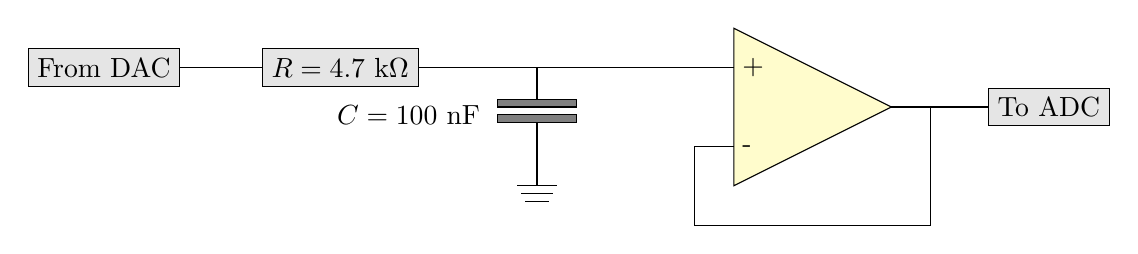
\begin{tikzpicture}[
	block/.style={draw,fill=gray!20!white},
	auto
	]
		\draw[fill=yellow!20!white] (0,1) -- (0,-1) -- (2,0) -- cycle;
		\path (0,0.5) node[inner sep=0.1cm,right] (opamp+) {+};
		\path (0,-0.5) node[inner sep=0.1cm,right] (opamp-) {-};
		\draw (opamp-) -- (-0.5,-0.5) -- (-0.5,-1.5) -- (2.5,-1.5) -- (2.5,0) -- (2,0);
		\path (4,0) node[block] (toadc) {To ADC};
		\draw (2.5,0) -- (toadc);
		
		\path (-5,0.5) node[block] (r) {$R=4.7$ k$\Omega$};
		\draw (r) -- (opamp+);
		\path (-8,0.5) node[block] (in) {From DAC};
		\draw (in) -- (r);
		
		\draw[fill=gray] (-3,0) rectangle (-2,0.1);
		\draw[fill=gray] (-3,-0.2) rectangle (-2,-0.1);
		\path (-3.1,-0.1) node[fill=white,left] (c) {$C=100$ nF};
		\draw (-2.5,0.5) -- (-2.5,0.1);
		\draw (-2.5,-0.2) -- (-2.5,-1);
		\draw (-2.75,-1) -- (-2.25,-1);
		\draw (-2.7,-1.1) -- (-2.3,-1.1);
		\draw (-2.65,-1.2) -- (-2.35,-1.2);
		
	\end{tikzpicture}
	\caption{Electrical schematic for measuring the open-loop response of a low-pass filter.}
	\label{fg:openLoopSchematic}
\end{figure}
The buffer is needed because of the relatively high input impedance of the ADC evaluation board.  

The folder ``Open loop measurement example'' contains the necessary files.  To measure the open loop response, run the script \verb|measureOpenLoopLinear|.  This will measure the response to modulations in the frequency range 10 Hz to 10 kHz using a 32 $\mu$s DAC update period and ADC sample period.  The data will be saved in the file ``Open loop response.mat'' in the same folder.  To analyze the resulting data, run the file \verb|calcOpenLoop|.  This program will fit sine curves to the measured ADC voltages, using the modulation parameters to constrain the fit, to get the amplitude and phase shift.  The amplitude and phase shift is then used in a fit to a second-order frequency response in addition to the known low-latency filter response (see the ADC datasheet).  The second output argument from the \verb|calcOpenLoop| function, pFilter, is a vector with the second order response parameters
\begin{equation}
G(\omega) = \frac{G(0)}{1+i\frac{\omega}{\omega_1} -\frac{\omega^2}{\omega_2^2}}
\label{eq:secondOrderResponse}
\end{equation}
where $\text{pFilter}(1) = G(0)$, $\text{pFilter}(2) = \omega_1/(2\pi)$, and $\text{pFilter}(3) = \omega_2/(2\pi)$.  $G(0)$ should be very close to 1, and for the RC filter in Fig.~\ref{fg:openLoopSchematic} $\omega_1 \approx 338$ Hz.  The term $\omega_2$ is included to account for non-ideal effects in the buffered RC filter.  An example of the open loop measurement is shown in Fig.~\ref{fg:openLoopMeas}.
\begin{figure}[htbp]
	\centering
	\includegraphics[width=10cm]{OpenLoop.pdf}
	\caption{Bode plot of the open loop response of the buffered RC filter when measuring using the ADC with a low-latency filter and 512x OSR.  Blue circles are from measurements, red dashed line is a fit to $G(\omega)M(\omega)$.  Here, $G_0 = 0.9945$, $\omega_1/(2\pi) = 324.7$ Hz, and $\omega_2/(2\pi) = 2611$ Hz.  \textbf{(a)} Amplitude of the response as a function of frequency.  \textbf{(b)} Phase shift as a function of frequency.}
	\label{fg:openLoopMeas}
\end{figure}
Here, the ADC filter was set to a low-latency filter with 512x OSR.  From equation 4 on the ADC datasheet, the filter response is
\begin{equation}
M(\omega=2\pi f) = e^{-2\pi i f T_s} \left|\frac{\sin\left(\frac{32\pi f}{f_{\rm CLK}}\right)}{32\sin\left(\frac{\pi f}{f_{\rm CLK}}\right)}\right|^5 \left|\frac{\sin\left(\frac{32 N_s\pi f}{f_{\rm CLK}}\right)}{N_s\sin\left(\frac{32\pi f}{f_{\rm CLK}}\right)}\right|
\label{eq:MeasurementResponse}
\end{equation}
where $f_{\rm CLK}$ is the ADC master clock frequency (16 MHz), and $N_s$ is the second-stage oversampling ratio equal to the OSR setting divided by 32, $\mathrm{OSR}/32$.

Using the measured $G(\omega)$, the response of the servo to any set of gains for Eq.~\eqref{eq:controlLaw} can now be calculated.  Alternatively, one can calculate the gains needed to approximate a given response.  Suppose that we want our closed loop response to be $T(\omega) ^{-1} = 1+1i\omega/\omega'$ where $\omega'$ is the target cut-off frequency for a low-pass filter -- i.e., we want to change the cut-off frequency of our RC filter.  If the control law is $K(\omega)$, then the closed-loop response is
\begin{equation}
	T(\omega) = \frac{G(\omega)K(\omega)M(\omega)}{1+G(\omega)K(\omega)M(\omega)}
	\label{eq:closedLoopResponse}
\end{equation}
and thus we can calculate the needed control law if we know $T(\omega)$:
\begin{align}
	K(\omega) &= \frac{T(\omega)}{1-T(\omega)}G^{-1}(\omega)M^{-1}(\omega)\notag\\
	&= \left(\underset{K_p}{\underbrace{\frac{\omega'}{\omega_1 G(0)}}} + \underset{K_i}{\underbrace{\frac{\omega'}{G(0)}}}\frac{1}{i\omega} + \underset{K_d}{\underbrace{\frac{\omega'}{\omega_2^2G(0)}}}i\omega\right)M^{-1}(\omega).
	\label{eq:loopShaping}
\end{align}
Due to the complex nature of $M(\omega)$, in calculating the gain parameters of $K(\omega)$ we typically assume that $M(\omega)\approx 1$ which is accurate for $\omega T_s\ll 1$.  Simpler measurement responses could be incorporated into $G(\omega)$ to form an effective open-loop response $\tilde{G}(\omega) = G(\omega)M(\omega)$.  Note that to convert from a continuous description of the control law to a discrete version time needs to be measured in units of $T_s$.

The script file \verb|measureClosedLoopLinear| measures the closed-loop response of the buffered RC filter using four different target cut-off frequencies for $T(\omega)$: $\omega'/(2\pi) = 250,500,1000,\text{ and }2000$ Hz.  The data collected by this script can be analysed using the file \verb|calcClosedLoop|, which uses the function \verb|PIDsim| to model the system response.  Results are shown in Fig.~\ref{fg:closedLoopResponse}.
\begin{figure}[htbp]
	\centering
	\includegraphics[width=10cm]{ClosedLoop.pdf}
	\caption{Bode plot of the closed loop response with different target low-pass cut-off frequencies of 250 Hz (blue), 500 Hz (yellow), 1000 Hz (green), and 2000 Hz (red).  Open circles are the measured response, and solid lines are the modelled response based on the open loop parameters and the servo controller's PID calculation.  \textbf{(a)} Amplitude of the signal as a function of frequency.  \textbf{(b)} Phase shift of the signal as a function of frequency.}
	\label{fg:closedLoopResponse}
\end{figure}
As both the ADC and DAC are well-characterized, and the FPGA latency is well-known, the model of the controller is a good match to the measurements.  This model can thus be used to determine the response of the controller to any set of PID gains or when connected to a system with different open loop dynamics.  We define the closed-loop response as
\[
T(\omega) = \frac{L(\omega)}{1+L(\omega)}
\]
where $L(\omega)$ is the so-called loop gain equal to
\[
L(\omega) = K(\omega)H(\omega)G(\omega)M(\omega)
\]
where $G(\omega)$ is the open-loop response, $M(\omega)$ is the measurement response, $H(\omega) = e^{-i\omega T_{\rm lag}}$ is the phase shift due to the FPGA latency of $T_{\rm lag} \approx 6$ $\mu$s.  The control law $K(\omega)$ is modelled as
\begin{equation}
K(\omega) = \left[\left(K_p+\frac{K_i}{2}+K_d\right) + \left(-K_p+\frac{K_i}{2}-2K_d\right)z^{-1} + K_dz^{-2}\right]\left[1-z^{-1}\right]^{-1}
\label{eq:discreteControlLaw}
\end{equation}
where $z^{-1} = \exp\left(-i\omega T_s\right)$.

\end{document}